\section{Data-dependent, task-optimized streams}
\label{sec:data_dep_streams}

This section aims to solve the problem of finding the ``best'' (data-dependent) stream possible,
given a data set and an error metric. This stream is important because it serves both as a benchmark
and a source of insights for other, more practical streams. One way to define the best stream could
be the stream that incurs the minimum error at every point. However, in trying to realize such a
stream, our experience has been that such a stream does not exist. Assume otherwise that the optimal
stream exists, then by its definition, it must be possible to construct it using the following
greedy algorithm: start with a pool of all chunks, pick the one that minimizes the error, remove it
from the pool of chunks, and repeat until the pool is empty. Running this algorithm, we have noticed
that there can be a situation in which the next chunk that minimizes the error is on a low-order bit
plane of a very fine-scale coefficient, which contributes little to the reconstructed function. The
error is minimized because it is kept approximately constant. In this case it is actually better to
pick a chunk that increases the error, but otherwise contributes a lot more to the reconstructed
function. In optimization terms, it is necessary to move in a direction that increases the error to
avoid getting stuck in a local minima.

The ``best'' stream for an error metric can also be defined as the stream such that the area bounded
by its plotted error curve and the horizontal axis is smallest. However, the usefulness of such a
definition is limited in practice, because a stream should be able to be terminated at any point and
still be expected to produce as small of an error as possible. Instead, we observe that the greedy
algorithm stated in the paragraph above can be slightly modified to avoid the problem of being stuck
in local minima. We start with a set consisting of all the chunks, and an empty stream, which will
be built from back to front. In each step, the chunk whose removal from the set has the least impact
on the error is removed and inserted to the beginning of the stream. This algorithm solves the
problem of unimportant chunks being picked too early in the original algorithm, because here, being
picked early means they would be at the end of the stream, instead of the beginning.

In our experience, however, the back-to-front greedy algorithm is too costly in practice. Ignoring
all the steps done in each iteration, this algorithm amounts to an $n^2$-iteration, 2-level nested
loop, where $n$ is the number of chunks. In 2D, with a $256^2$ data set, a chunk size that spans
$16$ coefficients, and $16$ bits of quantization, the total number of chunks would be $n=65536$, and
$n^2$ would be in the billions, which we have found to be prohibitively large. We have therefore
adopted a simplified version of this algorithm, where only one pass through the chunks are needed.
Our modified algorithm disables (sets to zero) a new chunk in each iteration, computes and records
the error due to that chunk missing, and finally re-enables the chunk at the end of the iteration.
After $n$ iterations, each chunk has an associated weight, that is its impact on the error. The
``optimal'' stream, then, is simply a sorted list of chunks, in decreasing order of weights. In our
experience, this simplified algorithm brings the running time down from days to minutes, while
sacrificing none of the quality of the output stream.

For each quantity of interest, such as histogram or isocontour, we can now compute a stream that is
optimized for that quantity, using the algorithm above, and the corresponding error metric to the
quantity of interest. This stream is to be viewed as an empirical upper-bound on all possible
streams that aim to minimize the same error metric. Since each quantity is typically associated with
a task (e.g., the quantity ``isocontour'' corresponds to the task ``visualizing an isocontour''), we
also call such streams task-optimized. The list of task-optimized streams studied in this paper
includes \emph{rmse-optimized} (Section [REF]), \emph{gradient-optimized} (Section [REF]),
\emph{laplacian-optimized} (Section [REF]), \emph{histogram-optimized} (Section [REF]), and
\emph{isocontour-optimized} (Section [REF]), for a wide variety of data sets.

\textbf{Minimizing function error in $L_2$} The most fundamental task is that of reconstructing the
function itself, using a common error metric such as the root-mean-square error (RMSE). For each
data set, we use the aforementioned $O(n)$ greedy algorithm to construct an \emph{rmse-optimized}
stream. In Section \ref{sec:motivation} we have seen that the \emph{by wavelet norm} performs the
best among the data-agnostic streams. To see how the \emph{rmse-optimized} stream, which is
data-dependent, compares to the data-agnostic streams, we plot all four streams together in Figure
\ref{fig:rmse-optimized}. It can be seen that the difference between \emph{by wavelet norm} and
\emph{rmse-optimized} is negligible. This result is expected, because \emph{by wavelet norm} and
\emph{rmse-optimized} both order the chunks according to their contribution to the function in $L_2$
sense, with \emph{rmse-optimized} taking into account the actual values of the bits. This difference
has little effect in this case, because, as leading zero bits are removed, the rest of the bits (of
the wavelet coefficients) are known to be distributed approximately uniformly among $0$ and $1$ for
wavelet coefficients [CITE].

\begin{figure}
  \centering
	\subcaptionbox{Boiler}
  {\includegraphics[width=0.48\linewidth]{img/rmse/rmse-optimized-boiler.pdf}}
	\subcaptionbox{Diffusivity}
 	{\includegraphics[width=0.48\linewidth]{img/rmse/rmse-optimized-diffusivity.pdf}}
	\subcaptionbox{Euler}
 	{\includegraphics[width=0.48\linewidth]{img/rmse/rmse-optimized-euler.pdf}}
	\subcaptionbox{Turbulence}
 	{\includegraphics[width=0.48\linewidth]{img/rmse/rmse-optimized-turbulence.pdf}}
	\subcaptionbox{Plasma}
 	{\includegraphics[width=0.48\linewidth]{img/rmse/rmse-optimized-plasma.pdf}}
	\subcaptionbox{Velocity-z}
 	{\includegraphics[width=0.48\linewidth]{img/rmse/rmse-optimized-velocityz.pdf}}
 	\caption{Root-mean-square error of reconstructed functions for the three data-agnostic streams
 	defined in Section \ref{sec:motivation}, and the \emph{rmse-optimized} stream. Lower is better.
 	The streams are truncated to highlight the differences, without omitting important information.
 	\emph{rmse-optimized} performs best, followed closely by \emph{by wavelet norm} and \emph{by bit
 	plane}.}
 	\label{fig:rmse-optimized}
\end{figure}

% \paragraph*{Fine-to-coarse greedy algorithm} utilizes full dataset to construct the stream.
% Moreover, if we wanted to precompute stream order which could be utilized during query, we would
% have access to whole data set and could compute this stream. The algorithm is in principle a reverse
% of the previous approach \hb{perhaps the order was switched?}, the stream is constructed by starting with full data set and one by one
% disabling the chunks. At each step, a chunk with smallest errorr impact is disabled (TODO: more
% detail). This algorithm is still of greedy nature as it makes only locally optimal choice. The
% running time of this algorithm is $O(n^3)$ as we start with $n$ chunks and at each streaming step
% decrease the chunk count by one. The cube factor comes from the need to perform inverse wavelet
% transform and compute the error for each chunk.

% \begin{algorithm}
%   \KwData{slice, unordered list of chunks}
%   \KwResult{ordered list of chunks with decreasing error}
%   orderedChunks = $\emptyset$\;

%   \While{$|$chunks$| \ne 0$}{
%    smallestChunk = front(chunks)\;
%    \For{chunk $\in$ chunks}{
%      sliceCopy = slice\;
%      disableChunk(sliceCopy, chunk)\;
%      error = computeError(sliceCopy, slice)\;
%      \If{error $<$ error(smallestChunk)}{
%        smallestChunk = chunk\;
%      }
%    }

%    disableChunk(slice, smallestChunk)\;
%    chunks = chunks $\setminus$ smallestChunk\;
%    orderedChunks = orderedChunks $\cup \{$smallestChunk$\}$\;
%   }
%   \caption{Fine-to-coarse stream optimization algorithms. \hb{use symbols for unordered / ordered sets? this would be strict total ordering nor partial ordering, right? 
%   depending upon that, $\cup$ may or may not maintain ordering.  
%   what is the `slice' in input? }}
% \end{algorithm}

% \begin{figure}
%   \centering
%   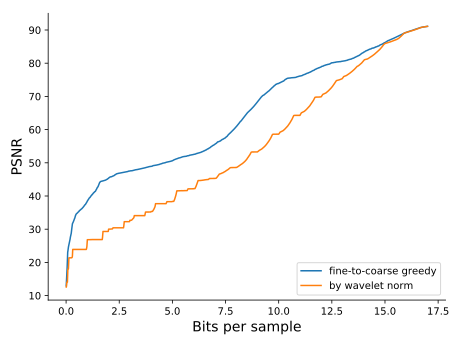
\includegraphics[width=0.48\linewidth]{img/figure4_new/rmse-miranda-viscosity}
%   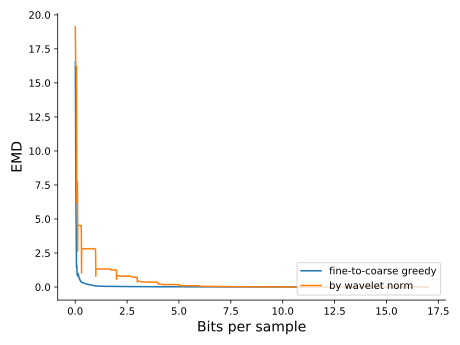
\includegraphics[width=0.48\linewidth]{img/figure4_new/histogram-miranda-viscosity}
%   \caption{Comparison of fine-to-coarse and by wavelet norm streams on Miranda viscosity data set.
%             On the left is stream optimized for PSNR (higher is better) and on the right for
%             histogram (lower is better). Despite using larger block size for the greedy stream ($16
%             \times 16$) due to performance reasons, it still significantly outperforms the by
%             wavelet norm stream for both quantities.}
% \end{figure}

% \paragraph*{Coarse-to-fine greedy algorithm} starts with no data and the initial error is computed
% with respect to the full data set. Then it takes a list of all chunks in the dataset, computes the
% error as if the chunk was enabled, and picks the chunk with the highest absolute difference in the
% error with respect to the current error.  We use absolute difference to avoid the case where the
% error difference is zero or negative, which would result in a long stream of chunk that do not
% decrease the error significantly. \ptb{I am not sure in understand the previous sentence} This
% assumption reflects the expectation of more data meaning better result. Similarly to the
% coarse-to-fine algorithm, the running time is still $O(n^3)$.

% Since the fine-to-coarse greedy stream outperforms \hb{needs to be pointed out using the figures}
% the coarse-to-fine stream we further investigate possible runtime optimizations. Surprisingly,
% performing only the first round of chunk error calculation and then sorting those chunks by the
% error closely matches the full greedy algorithm. This simple optimization reduces the time
% complexity to $O(n^2)$ and thus makes it more practical. We use this greedy scheme throught our
% evaluation named \emph{fully adpative} stream.

% \begin{figure}
%   \centering
%   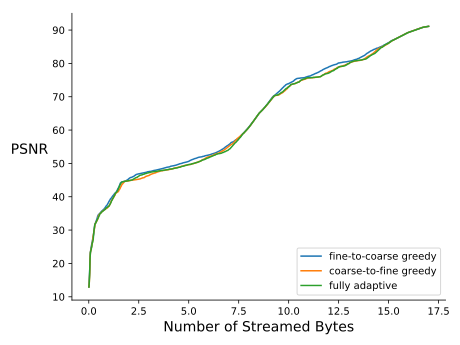
\includegraphics[width=0.48\linewidth]{img/figure6/rmse-miranda-viscosity}
%   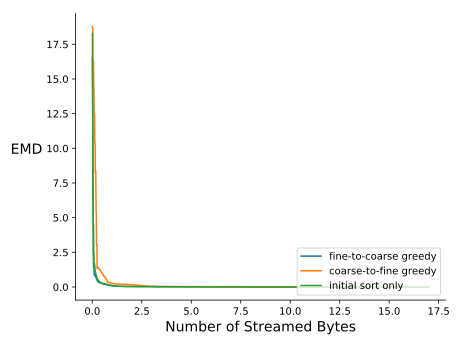
\includegraphics[width=0.48\linewidth]{img/figure6/histogram-miranda-viscosity}
%   \caption{The fully adaptive stream (fine-to-coarse with only initial sorting) closely
%             follows the coarse-to-fine and fine-to-coarse streams both for PSNR and histogram.}
% \end{figure}
